\appendix
\chapter{Sec'tiuni relevante din cod}
Clasele din fi'sierul $parsing.py$ aferente identific'arii unor 'intreb'ari complexe:

\begin{verbatim}
#----------class individuals-------------

class ListIndividuals(QuestionTemplate):
    target = Group(Pos("NN") | Pos("NNP") | Pos("NNS"), "target")
    optional_opening = Question((Pos("WP") | Pos("WDT"))
                       + Lemma("be") + Pos("DT"))
    regex1 = optional_opening \
             + Question(Lemma("individual") | Lemma("instance")) + \
             Pos("IN") + target + Question(Pos("."))
    regex2 = Question(Lemma("list") | Lemma("show") | Lemma("print")) \
             + target + \
             Question(Lemma("individual") | Lemma("instance"))
    regex = (regex1 | regex2)

    def interpret(self, match):
        algorithms = factory("Is" + match.target.tokens)
        return algorithms, "enum"

#---------------has-learning-method ------------

class GivenAlgorithmHasLearningMethod(QuestionTemplate):
    optional_opening = Question((Pos("WP") | Pos("WDT")) + Lemma("be") +\
                        Pos("DT"))
    regex1 = optional_opening + (Lemma("learn") + Lemma("method")) + \
             Pos("IN") + Algorithm() + Question(Pos("."))
    regex2 = Question(Lemma("list") | Lemma("show") | Lemma("print")) +\ 
             Algorithm() + (Lemma("learn") +\ 
             (Lemma("method") | Lemma("methods")))
    regex3 = Algorithm() + (Lemma("learn") + \ 
            (Lemma("method") | Lemma("methods")))
    regex = (regex1 | regex2 | regex3)

    def interpret(self, match):
        alg = HasLearningMethodReversed(match.algorithm)
        return alg, "enum"


#--------------- subclass off ----------------

class MySubclassOf(QuestionTemplate):
    target = Group(Pos("NN") | Pos("NNP"), "target")
    optional_opening = Question(Pos("WP") + Lemma("be") + Pos("DT"))
    regex1 = optional_opening +\ 
            Question(Lemma("subclass") | Lemma("family")) + \
             Pos("IN") + target + Question(Pos("."))
    regex3 = Question(Lemma("method")) + Question(Pos("IN")) + target
    regex2 = target + Question(Lemma("subclass"))
    regex = (regex1 | regex2 | regex3)

    def interpret(self, match):
        target = HasInstance(match.target.tokens, operator="")
        subclasses = IsSubclassOf(target)

        return subclasses, "enum"
        
#---------------not-------------------- 

class NotHaveLearningMethod(QuestionTemplate):
    regex = Question(Lemmas("algorithm that do not") +\ 
            (Lemma("have"))) +  LearningMethod(operator="MINUS ") +\  
            Question(Lemmas("learn method"))

    def interpret(self, match):
        alg = IsAlgorithm()
        alg_not = NotHasLearningMethod(match.learningmethod)
        return alg + alg_not, "enum"

#------------- and --------------------

class SolvesProblemAndHasLearningMethod(QuestionTemplate):
    regex = Question(Lemmas("algorithm that")) +\ 
            Question((Lemma("solve") | Lemma("resolve"))) + \
             LearningProblem(operator="AND") +\ 
             Question(Lemma("problem"))+\
             Question(Lemma("and")) +\ 
             Question(Lemma("use") | Lemma("have"))+
             LearningMethod(operator="AND") + \
             Question(Lemmas("learning method")) + \
             Question(Lemma("and")) + Question(Lemma("have")) +
             Question(Lemma("feature")) + Feature(operator="AND")

    def interpret(self, match):
        algorithms = IsAlgorithm()
        learning_methods = HasLearningMethod(match.learningmethod)
        learning_problems = SolvesLearningProblem(match.learningproblem)
        features = HasFeature(match.feature)
        return algorithms + learning_methods + learning_problems +\ 
                features, "enum"

# --------------- or---------------------

class AlgorithmSuitableForD1orD2(QuestionTemplate):
    regex = Lemma("algorithm") + Lemma("suitable") + Pos("IN") + 
            DataCharacteristic(name="dc1", operator="OR") + \ 
            Lemma("or") + DataCharacteristic(name="dc2", operator="OR") +
            Question(Lemmas("data characteristic"))

    def interpret(self, match):
        algorithm = IsAlgorithm()
        data_chr1 = SuitableFor(match.dc1)
        data_chr2 = SuitableFor(match.dc2)

        return algorithm + data_chr1 + data_chr2, "enum"

#--------------class of individual ---------

class WhatIs(QuestionTemplate):
    target = Group(Pos("NN") | Pos("NNP") | Pos("NNS") | Pos("VBG") 
        | Pos("FW") | Pos("JJR") | Plus(Pos("JJ") | Pos("NN")),"target")
    regex1 = target + Question(Lemma("type") | Lemma("class"))
    regex2 = Lemma("what") + Lemma("be") + Question(target) + \ 
            Question(Lemma("type") | Lemma("class"))
    regex3 = Question((Lemma("type") | Lemma("class")) + Pos("IN")) +\ 
            target
    regex = (regex1 | regex2 | regex3)

    def interpret(self, match):
        target = HasInstance(match.target.tokens, operator="")
        type = HasType(target)

        return type, "enum"
\end{verbatim}

Clasele implementate 'in $dsl.py$ pentru a sus'tine 'intreb'arile cu operatori logici:

\begin{verbatim}

class MinusFixedRelation(Expression):
    relation = None
    reverse = False

    def __init__(self, destination, reverse=None):
        if reverse is None:
            reverse = self.reverse
        super(MinusFixedRelation, self).__init__()
        if self.relation is None:
            raise ValueError("You *must* define the `relation` "
                             "class attribute to use this class.")
        self.relation = "MINUS " + self.relation
        self.nodes = copy(destination.nodes)
        self.head = destination.head
        self.decapitate(self.relation, reverse)


class FixedInstance(Expression):
    relation = None

    def __init__(self, data, operator):
        super(FixedInstance, self).__init__()
        if self.relation is None:
            raise ValueError("You *must* define the `instance` "
                             "class attribute to use this class.")
        self.relation = 
            encoding_flexible_conversion(operator + self.relation)
        self.add_data(self.relation, data)

class HasInstance(FixedInstance):
    relation = u"FILTER"

    def __init__(self, data, operator):
        super(HasInstance, self).__init__(data, operator)

\end{verbatim}

Metoda din $PelletService$, responsabil'a pentru ob'tinerea rezultatelor cu ajutorul libr'ariei Pellet:

\begin{verbatim}

private String runQuery(Query q) {

    QueryExecution qe = 
        SparqlDLExecutionFactory.create(q, ontology.getOntology());

    ByteArrayOutputStream catcher = new ByteArrayOutputStream();
    PrintStream PS = new PrintStream(catcher);
    PrintStream old = System.out;
    System.setOut(PS);

    ResultSet rs = qe.execSelect();
    ResultSetFormatter.outputAsJSON(rs);

    System.setOut(old);

    String warning;
    String result = catcher.toString();
    if (result.contains("WARN")) {
        String[] results = result.split("\n", 2);
        warning = results[0];
        String[] splitString = warning.split("\\[");
        warning = splitString[splitString.length - 1];
        warning = warning.substring(warning.indexOf(' ') + 1);
        throw new ResponseStatusException(HttpStatus.NOT_FOUND,
                        cleanResult(warning), new BusinessException());
    }
    result = cleanResult(result);
    return result;

}
\end{verbatim}
\chapter{Alte informa'tii relevante}
'In aceast'a anex'a se prezint'a lista complet'a a 'intreb'arilor/cerin'telor acceptate de agentul explicativ, grupate dup'a scopul lor.

\begin{enumerate}
    \item Afi'sarea instan'telor clasei <class\_name>. 
    
    % \begin{center}
    {\it
    "What are the instances of <class\_name>?"
    
    "Which are the individuals of <class\_name>?"
    
    "individuals of <class\_name>"
    
    "instances of <class\_name>"
    
    "print <class\_name> individual/s"
    
    "print <class\_name> instance/s" 
    
    "show <class\_name> instance/s"
    
    "show <class\_name> individual/s"
    
    "list <class\_name> individual/s"
    
    "list <class\_name> instance/s"
    }
    % \end{center}

\item Afi'sarea metodelor de 'inv'a'tare ale unui algoritm <algorithm\_individual> .

{\it
    "<algorithm\_individual> learning method/s"
    
    "What are the learning method/s of <algorithm\_individual>?"
    
    "print <algorithm\_individual> learning method/s"
    
    "list <algorithm\_individual> learning method/s"

}

\item Afi'sarea avantajelor unui algoritm <algorithm\_individual> .

{\it
    "What are the advantages of <algorithm\_individual>?"
    
    "list <algorithm\_individual> advantages"
    
    "<algorithm\_individual> advantages"
}

\item Afi'sarea dezavantajelor unui algoritm <algorithm\_individual> .

{\it
    "What are the disadvantage/s of <algorithm\_individual>?"
    
    "list <algorithm\_individual> disadvantage/s"
    
    "print <algorithm\_individual> disadvantage/s"
    
    "print <algorithm\_individual> disadvantage/s"
    
    "<algorithm\_individual> disadvantage/s"
}

\item Afi'sarea rezultatelor de performan't'a ale unui algoritm <algorithm\_individual> .

{\it

    "What are the performance result/s of <algorithm\_individual>?"
    
    "list <algorithm\_individual> performance result/s"
    
    "print <algorithm\_individual> performance result/s"
    
    "<algorithm\_individual> performance result/s"
}
    
\item Afi'sarea parametrilor unui algoritm <algorithm\_individual>.

{\it

    "What are the parameters of <algorithm\_individual> ?"
    
    "list <algorithm\_individual>  parameters"
    
    "print <algorithm\_individual>  parameters"
    
    "<algorithm\_individual>  parameters"
}
\item Afi'sarea caracteristicilor feature-urilor algoritmului <algorithm\_individual> .

{\it
    "What are the feature characteristics of <algorithm\_individual> ?"
    
    "list <algorithm\_individual>  feature characteristic/s"
    
    "<algorithm\_individual>  feature characteristic/s"
}
\item Provenien'ta instan'tei <individual>.

{\it
    "<individual> provenance"
}
    
\item Afi'sarea problemei rezolvate de algoritmul <algorithm\_individual>.

{\it
    "What learning problem does <algorithm\_individual> solve?"
    
    "list problems solved by <algorithm\_individual>"
}
\item Afi'sarea subclaselor clasei <class\_name>.

{\it
    "<class\_name> subclass"
    
    "What is the subclass of <class\_name>?"
 }   
\item Afi'sarea clasei de apartenen't'a a individului <individual>.

{\it
    "what is <individual>"
    
    "<individual> type"
    
    "<individual> class"
    
    "type of <individual>"
    
    "class of <individual>"
 }   
\item Afi'sarea algoritmilor care nu au metoda de 'inv'a'tare <learning\_method>.

{\it
    "algorithm/s that do/does not have <learning\_method>"
    
    "algorithm/s that do/does not have <learning\_method> learning method"
    
    "algorithm/s that do/does not use <learning\_method>"
        
    "algorithm/s that do/does not use <learning\_method> learning method"
 }  

\item Afi'sarea algoritmilor care rezolv'a problema <solved\_problem> 'si au metoda de 'inv'a'tare <learning\_method> 'si au caracteristica <feature>.

{\it
    "algorithm that solve <solved\_problem> problem and have <learning\_method> learning method and have feature  <feature>"
    
    "algorithm that solve <solved\_problem> problem and have <learning\_method> and have feature  <feature>"
    
    "algorithm that solve <solved\_problem> problem and have <learning\_method> and have  <feature>"
    
    "algorithm that solve <solved\_problem> and have <learning\_method> and have  <feature>"
}


\item Afi'sarea algoritmilor care sunt potrivi'ti pentru <data\_characteristic\_1> sau <data\_characteristic\_2>.

{\it
    "algorithm that have  <data\_characteristic\_1> or <data\_characteristic\_2>"
    
    "algorithm suitable for <data\_characteristic\_1> or <data\_characteristic\_2>",
}

\item Afi'sarea comentariului asociat individului <individual>.

{\it
    "show details of <individual>"
    
    "list definitions of <individual>"
    
    "print definition of <individual>"
    
    "define <individual> individual"
    
    "tell me more about <individual>"
}
\end{enumerate}

\chapter{Lucr'ari publicate (dac'a exist'a)}

Agentul explicabil pentru 'inv'a'tare automat'a descris 'in aceast'a lucrare a fost prezentat 'si 'in articolul "Towards Explainable Machine Learning Using  Natural Language Processing and Ontologies". Articolul este trimis la "IEEE 15th International Conference on
Intelligent Computer Communication and Processing (ICCP 2019)" 'si se afl'a in curs de verificare. Cu o variant'a restr\ia ns'a a acestuia am participat la "Conferin'ta 'Stiin'tific'a a Studen'tilor Sec'tiilor de Calculatoare 2019".
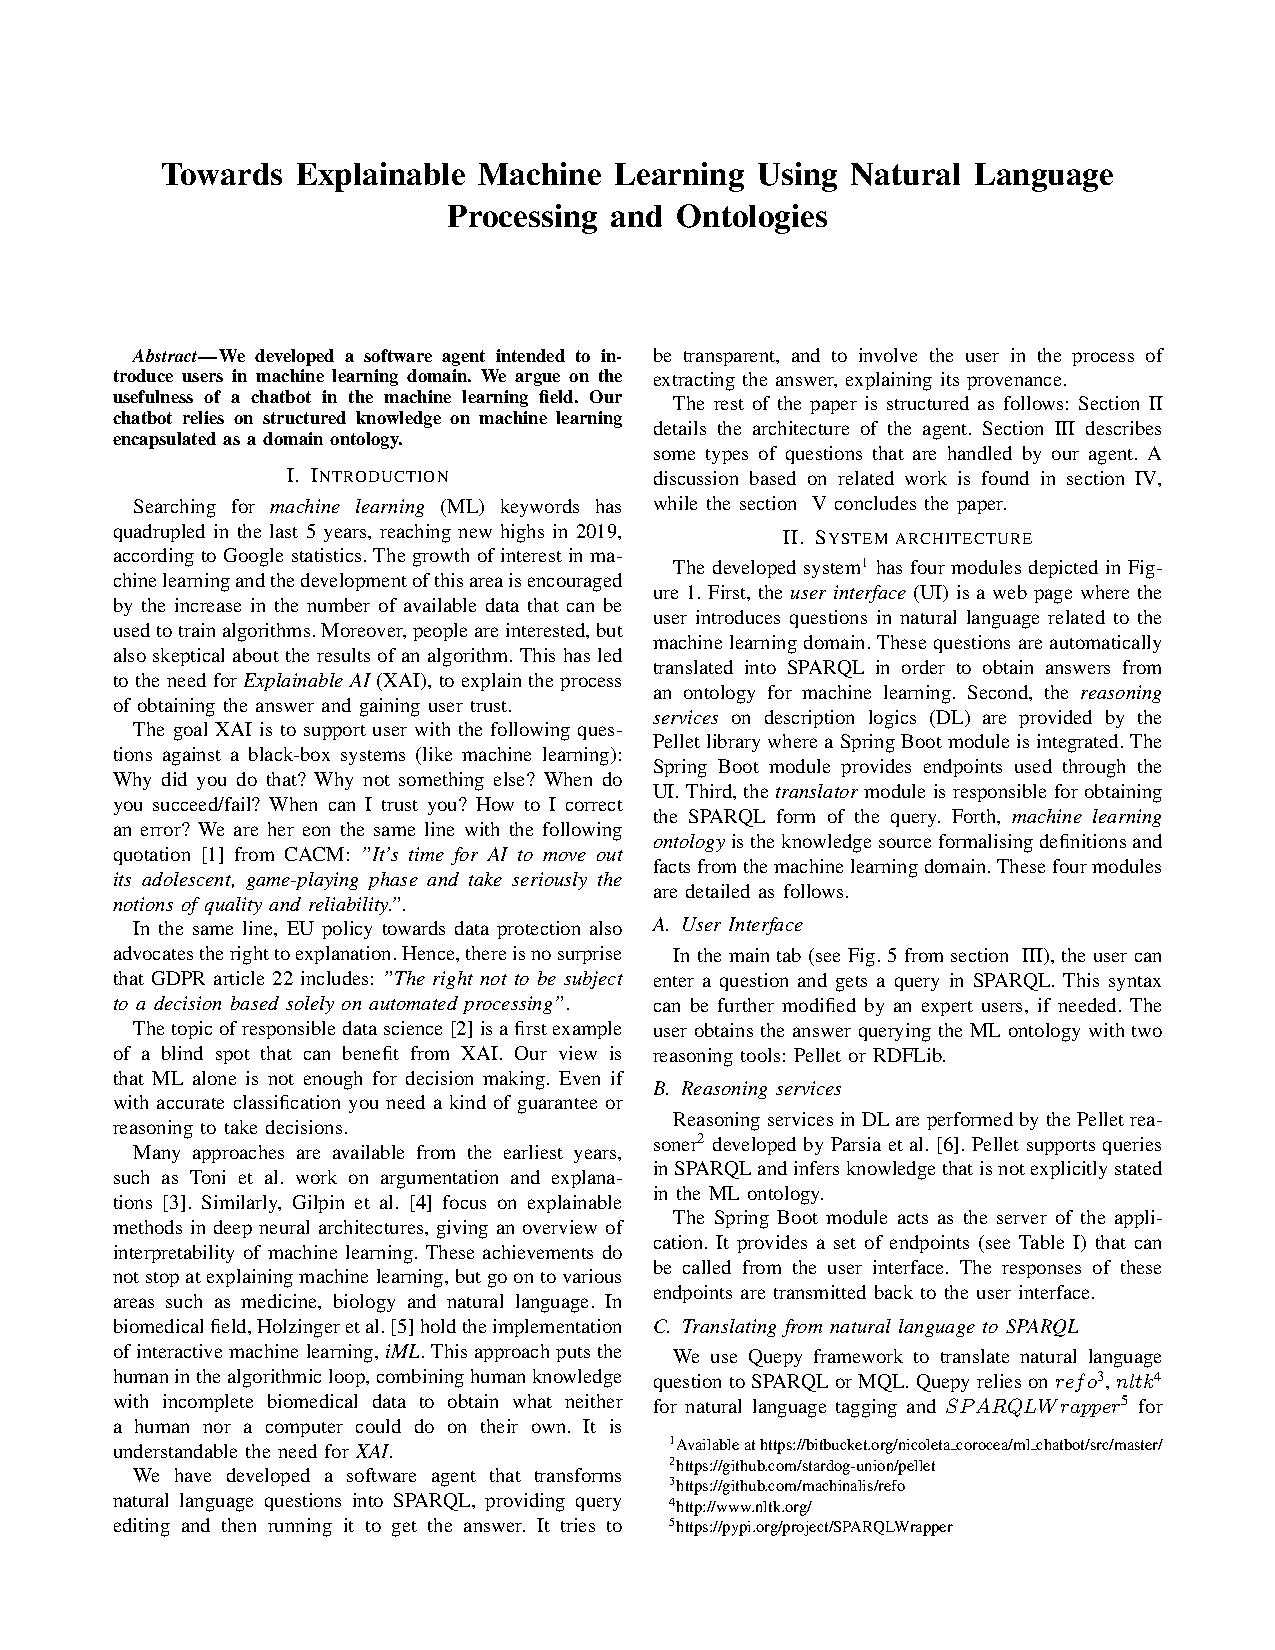
\includepdf[pages=-,pagecommand={},width=\textwidth]{articol_extins.pdf}
